\documentclass[11pt,a4paper]{article}

\usepackage{amsmath}
\usepackage{graphicx}
\usepackage{epstopdf}

\title{AMTH250 \\ Assignment 3}
\author{Mark Villar}

\begin{document}

\maketitle

Here is a random $4 \times 4$ matrix:
\begin{verbatim}
	0.062629   0.064961   0.499433   0.533246
	0.103524   0.876906   0.561583   0.363536
	0.427636   0.058570   0.983110   0.039192
	0.140933   0.452862   0.482425   0.439356
\end{verbatim}
and here is a graph of Brownian motion:

\begin{figure}[!ht]
	\begin{center}
		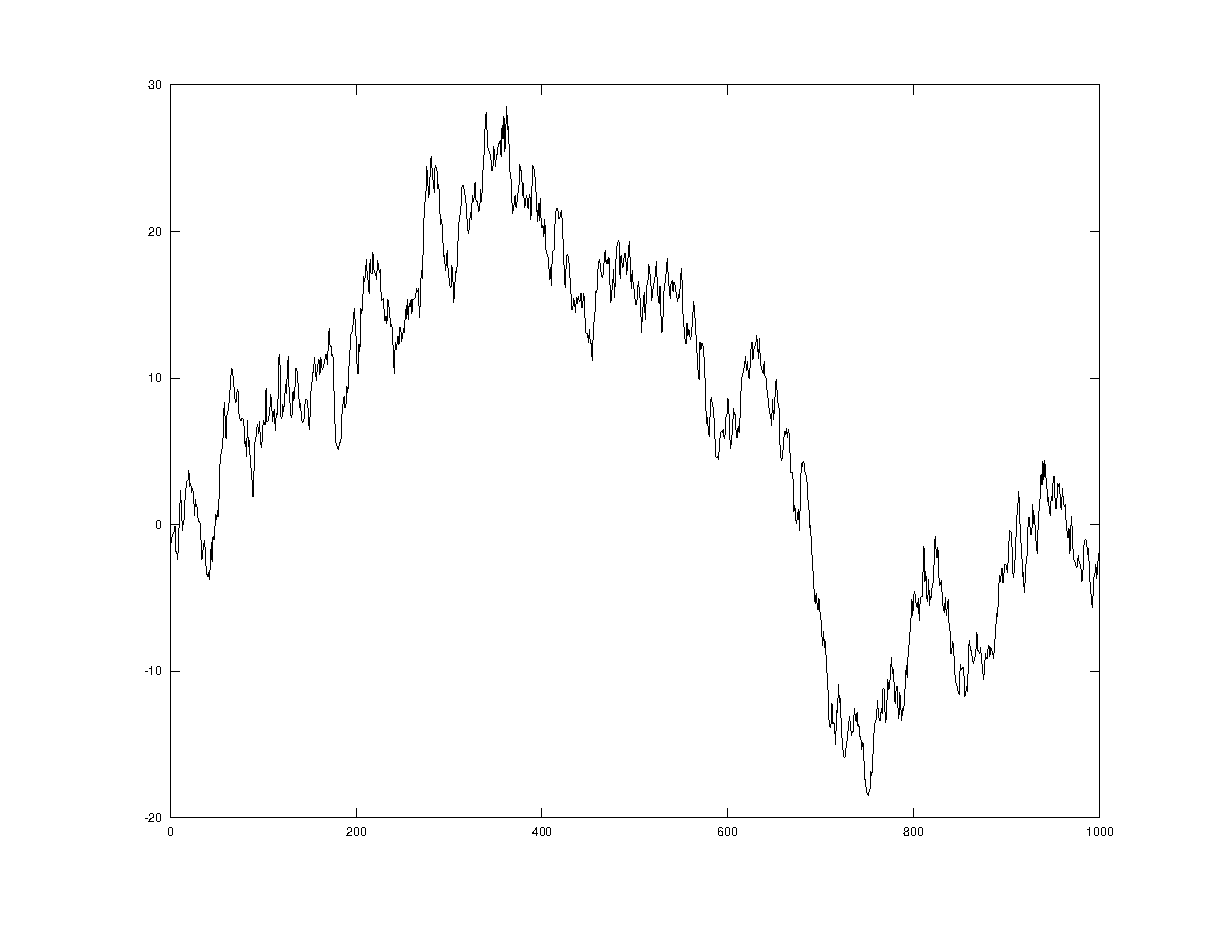
\includegraphics[width=0.8\textwidth]{brown.eps}
		\caption{Brownian Motion}
	\end{center}
\end{figure}

\end{document}